\graphicspath{{5Fractals/asy/}}

\section{Fractal Geometry}

\subsection{Natural Geometry, Self-similarity and Fractal Dimension}\label{sec:fracdefn}

The objects of classical geometry (lines, curves, spheres, etc.) tend to seem flatter and less interesting as one zooms in: at small scales, every differentiable curve looks like a line segment! By contrast, real-world objects tend to exhibit greater detail at smaller scales. A seemingly spherical orange is dimpled on closer inspection: is its surface area that of a sphere, or is the area greater due to the dimples? What if we zoom in further? Under a microscope, the dimples in the orange are seen to have minute cracks and fissures. With modern technology, we can `see' almost to the molecular level; what does \emph{surface area} even mean at such a scale?

\boldinline{The Length of a Coastline} In 1967 Benoit Mandelbrot asked a related question in a now-famous paper, \emph{How Long Is the Coast of Britain?\ Statistical Self-Similarity and Fractional Dimension.} His essential point was that this question has no simple answer:\footnote{%
	The official answer from the Ordnance Survey (the UK government mapping office) is, `It depends.' The all-knowing CIA states 7723 miles, though offers no evidence as to why.%
} Should one measure by walking along the mean high tide line? But where is this? Do we `walk' round every pebble? Do we skirt every grain of sand? Every molecule? As the scale of consideration shrinks, the measured length becomes absurdly large. Here is a sketch of Mandelbrot's approach.\footnote{%
	For more detail see the Fractal Foundation's \href{http://fractalfoundation.org/OFC/OFC-10-4.html}{website.} Mandelbrot coined the word \emph{fractal}, though he didn't invent the concept from nothing. Rather he applied earlier ideas of Hausdorff, Minkowski and others, and observed how the natural world contains many examples of fractal structures.%
}
\begin{itemize}
  \item Given a ruler of length $R$, let $N$ be the number required to trace round the coastline when laid end-to-end.
  \item Plot $\log N$ against $\log (1/R)$ for several sizes of ruler. The data suggests a straight line!
  \[
  	\log N\approx \log k+D\log(1/R)=\log (kR^{-D})\implies N\approx kR^{-D}
  \]
  The number $D$ is Mandelbrot's \emph{fractal dimension} of the coastline.
\end{itemize}

This notion of fractal dimension is purely empirical, though it does seem to capture something about the `roughness' of a coastline: the bumpier the coast, the greater its fractal dimension. For mainland Britain with its smooth east and rugged west coasts $D\approx 1.25$. Given its many fjords, Norway has a far rougher coastline and thus a higher fractal dimension $D\approx 1.52$.

\begin{example}{}{}
	As a sanity check, consider a smooth circular `coastline.'\par
	\begin{minipage}[t]{0.7\linewidth}\vspace{-8pt}
		Approximate the circumference using $N$ rulers of length $R$: clearly
		\[
			R=2\sin\frac\pi N
		\]
		As $N\to\infty$, the small angle approximation for sine applies,
		\[
			R\approx \frac{2\pi}N\implies N\approx 2\pi R^{-1}
		\]
	\end{minipage}
	\hfill
	\begin{minipage}[t]{0.29\linewidth}\vspace{-15pt}
		\flushright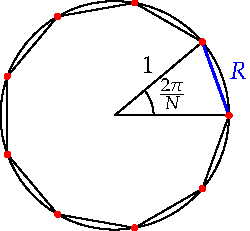
\includegraphics{self-sim-circle}
	\end{minipage}\medbreak
	where the approximation improves as $N\to\infty$. The fractal dimension of a circle is therefore $D=1$. The same analysis applies to any smooth curve (Exercise \ref{exs:fractaldiffcurve}).
\end{example}


\goodbreak


Our goal is to describe a related notion of fractional dimension for \emph{self-similar} objects. To help motivate the definition, recall some of the standard objects of pre-fractal geometry.\par
\begin{minipage}[t]{0.75\linewidth}\vspace{-3pt}
	\begin{description}
		\item[Segment] A \textcolor{Green}{segment} can be viewed as $N$ copies of itself each scaled by a factor $r=\frac 1N$.
		\item[Square] A \textcolor{blue}{square} comprises $N$ copies of itself scaled by a factor $r=\frac 1{\sqrt N}$.
		\item[Cube] A cube comprises $N$ copies of itself scaled by a factor $r=\frac 1{\sqrt[3]{N}}$.
	\end{description}\vspace{-5pt}
	In each case observe that $N=\left(\frac 1r\right)^D$ where $D$ is the usual dimension of the object (1, 2 or 3). Inspired by this, we make a loose definition.
\end{minipage}
\hfill
\begin{minipage}[t]{0.24\linewidth}\vspace{-12pt}
	\flushright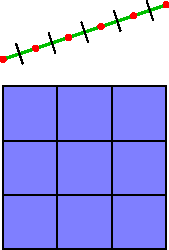
\includegraphics[scale=0.95]{self-sim-line}
\end{minipage}


\begin{defn}{}{selfsim}
	A geometric figure is \emph{self-similar} if it may be subdivided into $N$ similar copies of itself, each scaled by a magnification factor $r<1$. The \emph{fractal dimension} of such a figure is
	\[
		D:=\log_{1/r}N=\frac{\log N}{\log (1/r)}=-\frac{\log N}{\log r}
	\]
\end{defn}


\begin{example}{}{}
	The botanical pictures below offer some evidence for non-integer fractal dimension and for the idea that self-similarity is a natural phenomenon. The `tree' comprises $N=3$ copies of itself, each scaled by $r=0.4$. Its fractal dimension is therefore $D=-\frac{\log 3}{\log 0.4}\approx 1.199$.\par
	The fern has $N=7$ and $r=0.3$ for a fractal dimension $D=-\frac{\log 7}{\log 0.3}\approx 1.616$.
	\begin{center}
		\begin{tabular}{c@{\qquad\qquad}c}
			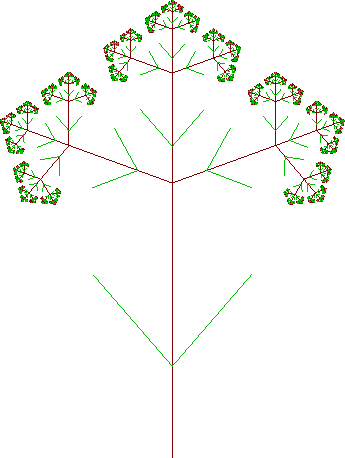
\includegraphics{tree2}
			&
			\href{http://www.math.uci.edu/~ndonalds/math161/fern-code.html}{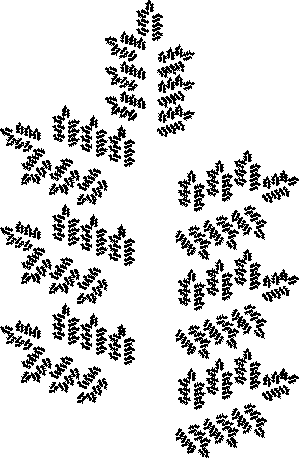
\includegraphics{tree3}}
			\\
			Tree fractal $D\approx 1.199$
			&
			Fern fractal $D\approx 1.616$
		\end{tabular}
	\end{center}
	With dimensions between 1 and 2, both objects exhibit an intuitive idea of fractal dimension: both seem to occupy more space than mere \emph{lines}, but neither has positive \emph{area}. Moreover, the fern seems to occupy more space---has higher dimension---than the tree. (The `trunk' and `branches' in the first picture aren't really part of the fractal and are drawn only to give the picture a skeleton.)
\end{example}


\goodbreak


\begin{example}{Cantor's Middle-third Set}{cantor}
	This famous example dates from the late 1800s.\footnotemark{}\par
	\begin{minipage}[t]{0.58\linewidth}\vspace{-5pt}
		Starting with the unit interval $C_0=[0,1]$, define a sequence of sets $(C_n)$ where $C_{n+1}$ is obtained by deleting the open `middle-third' of each interval in $C_n$; for instance
		\[
			C_1=\left[0,\frac 13\right]\cup\left[\frac 23,1\right]
		\]
		Cantor's set is essentially the limit of this sequence:
		\[
			\mathcal C:=\bigcap_{n=0}^\infty C_n
		\]
	\end{minipage}
	\hfill
	\begin{minipage}[t]{0.4\linewidth}\vspace{-7pt}
		\flushright
	\href{http://www.math.uci.edu/~ndonalds/math161/cantor-similar.html}{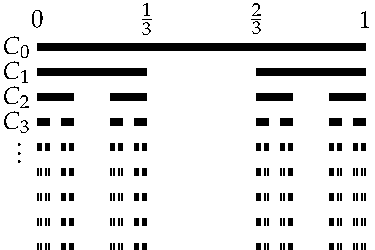
\includegraphics{cantor-set}}
	\end{minipage}
	\medbreak

	Cantor's set has several strange properties, none of which we establish rigorously.
	\begin{description}
	  \item[Zero length] The sum of the lengths of the disjoint sub-intervals comprising $C_n$ is $\operatorname{length}(C_n)=\left(\frac 23\right)^n$	since we delete $\frac 13$ of the remaining set at each step. It follows that
	  \[
	  	\forall n\in\N_0,\ \operatorname{length}(\mathcal C)\le \left(\frac 23\right)^n \implies \operatorname{length}(\mathcal C)=0
	  \]
	  We conclude that $\mathcal C$ contains no subintervals!
	  \item[Uncountability] There exists a bijection between $\mathcal C$ and the original interval $[0,1]$! (This issue is of limited interest to us, though you've likely encountered the notion elsewhere.)
	  \item[Self-similarity] Since $C_{n+1}$ consists of two copies of $C_n$, each shrunk by a factor of $\frac 13$ and one shifted $\frac 23$ to the right, we abuse notation slightly to write
		\[
			C_{n+1}=\frac 13C_n\cup\left(\frac 13C_n+\frac 23\right)
		\]
		`Taking limits,' Cantor's set is seen to comprise two shrunken copies of itself:
		\[
			\mathcal C=\frac 13\mathcal C\cup\left(\frac 13\mathcal C+\frac 23\right)
		\]
		In particular, its fractal dimension is $D=\frac{\log 2}{\log 3}\approx 0.631$.
	\end{description}

	The Cantor set has many generalizations:
	\begin{itemize}\itemsep0pt
	  \item Removing different fractions of every interval at each stage produces sets with other fractal dimensions. For instance, removing the 2\nd{} and 4\th{} fifths results in $D=\frac{\log 3}{\log 5}\approx 0.683$.
	  \item Higher-dimensional analogues include the \href{https://en.wikipedia.org/wiki/Sierpiński_triangle}{Sierpiński triangle} ($D=\smash{\frac{\log 3}{\log 2}}\approx 1.585$) and carpet (Examples \ref{ex:scarpet}, $D=\frac{\log 8}{\log 3}\approx 1.893$), and the Menger sponge ($D=\frac{\log 20}{\log 3}\approx 2.727$).
	\end{itemize}
\end{example}
\vspace{-5pt}

\footnotetext{%
	Henry Smith discovered this set in 1874 while investigating integrability (the `length' of a set was later formalized using \emph{measure theory}). Cantor's 1883 description focused on topological properties, with self-similarity being less of a concern.%
}

\goodbreak


\begin{example}{The Koch Curve and Snowflake}{koch}
	Another generalization of the Cantor set is produced as the limit of a sequence of curves.\par
	\begin{minipage}[t]{0.64\linewidth}\vspace{-4pt}
		\begin{itemize}\itemsep0pt
		  \item Let $K_0$ be a segment of length 1.
		  \item Replace the middle third of $K_0$ with the other two sides of an equilateral triangle to create $K_1$.
		  \item Replace the middle third of each segment in $K_1$ as before to create $K_2$.
		  \item Repeat \emph{ad infinitum.}
		\end{itemize}
		The resulting curve is drawn along with the \emph{Koch snowflake} obtained by arranging three copies around an equilateral triangle.\smallbreak
		
		The relation to the Cantor set should be obvious in the construction. Indeed if $K_0=[0,1]$, then the intersection of this with the Koch curve is the Cantor set itself!\smallbreak
		
		The Koch curve is self-similar in that it comprises $N=4$ copies of itself shrunk by a factor of $r=\frac 13$. Its fractal dimension is therefore $\frac{\log 4}{\log 3}\approx 1.2619$, between that of a line and an area.\smallbreak
		
		We may also consider the curve's length. Let $s_n$ be the number of segments in $K_n$, each having length $t_n$, and let $\ell_n=t_ns_n$ be the length of the curve $K_n$. It follows that
		\[
		  s_n=4^n,\quad t_n=\frac 1{3^n}
		  \implies \ell_n=\left(\frac 43\right)^n\to\infty
		\]
		The Koch curve is \emph{infinitely long}!
	\end{minipage}
	\hfill
	\begin{minipage}[t]{0.35\linewidth}\vspace{-15pt}
		\flushright
		\href{http://www.math.uci.edu/~ndonalds/math161/koch-anim.html}{
		\begin{tabular}{@{}c@{}}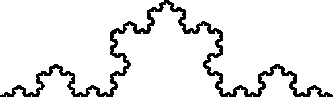
\includegraphics{koch}\\
			Koch Curve\\[8pt]
			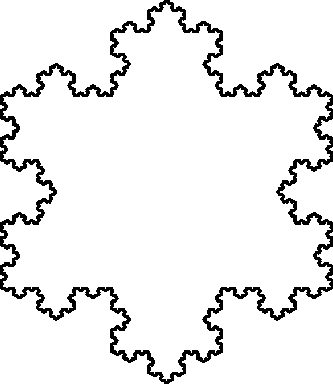
\includegraphics{koch2}\\
			Koch Snowflake\\[8pt]
			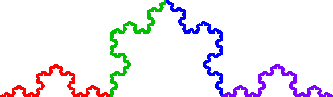
\includegraphics{koch3}\\
			Self-similarity
		\end{tabular}
		}
	\end{minipage}
\end{example}



\begin{exercises}
	\exstart By removing a constant middle fraction of each interval, construct a fractal analogous to the Cantor set but with dimension $\frac 12$.
	
	
	\begin{enumerate}\setcounter{enumi}{1}\itemsep2pt
		\item Prove that the area inside the $n\th$ iteration of the construction of the Koch snowflake is
		\[
			A_n=\frac{\sqrt 3}{4}\left(1+\frac 35\left[1-\left(\frac 49\right)^n\right]\right)
		\]
		\emph{The area inside the complete snowflake is therefore $\frac 85$ that of the original triangle.}
		
		
		\item\label{exs:fractaldiffcurve} Suppose $\vr(t)$, $t\in [0,1]$ is a regular (smooth) curve in the plane.
		\begin{enumerate}
	  	\item Use the arc-length formula $L=\int_0^1\nm{\vr'(t)}\,\dt$ together with Riemann sums and the linear approximation $\vr(t+\epsilon)\approx\vr(t)+\epsilon\vr'(t)$ with $\epsilon=\frac 1N$ to argue that
	  	\[
	  		L\approx\sum_{k=0}^{N-1}\nm{\vr\left(\frac{k+1}N\right)-\vr\left(\frac{k}N\right)} \tag{$\ast$}
	  	\]
	  	
	
	  	\item Suppose the curve is parametrized such that each segment on the right side of $(\ast)$ has the same length $R$. Prove that $L\approx NR$.\par
	  	(\emph{Any regular curve thus has fractal dimension 1 in the sense stated by Mandelbrot (pg.\,\pageref{sec:fracdefn})})
		\end{enumerate}
		
	\end{enumerate}
\end{exercises}


\clearpage




\subsection{Contraction Mappings \& Iterated Function Systems}

Thus far we have dealt informally with fractals where the whole consists of multiple pieces scaled by the same factor. In general we can mix up scaling factors. To do this, and to be more rigorous, it is helpful to borrow some language from topology.

\begin{defn}{}{}
	A \emph{contraction mapping} with scale factor $c\in[0,1)$ is a function $S:\R^n\to\R^n$ such that
	\[
		\forall x,y\in\R^n,\ \ \nm{S(x)-S(y)}\le c\nm{x-y}
	\]
\end{defn}

A contraction mapping moves inputs closer together. It should be clear that every such is continuous ($\lim x_n=y\Longrightarrow \lim S(x_n)=S(y)$). The main goal of this section is to see that fractals may be generated via repeated application of contraction mappings to an initial shape. We have already seen this!


\begin{example*}{\ref{ex:cantor}, mk.\,II}{}
	Consider the functions $S_1,S_2:\R\to\R$ where
	\[
		S_1(x)=\frac x3\qquad S_2(x)=\frac x3+\frac 23
	\]
	These are certainly contraction mappings (with scale factor $c=\frac 13$):
	\[
		\forall x,y\in\R,\ \ \nm{S_1(x)-S_1(y)}=\nm{S_2(x)-S_2(y)}=\frac 13\nm{x-y}
	\]
	More importantly, these functions \emph{define} the Cantor set: at each stage of its construction, we defined
	\[
		C_{n+1}:=S_1(C_n)\cup S_2(C_n)
	\]
	As the limit of this process, the self-similarity of the Cantor set can be expressed in the same manner: $\mathcal C=S_1(\mathcal C)\cup S_2(\mathcal C)$.\medbreak
	
	Surprisingly, it barely seems to matter what initial set $C_0$ was chosen. For example, we could start with the singleton set $C_0=\{0\}$, from which
	\[
		C_1=\{0,\tfrac 23\},\qquad C_2=\{0,\tfrac 29,\tfrac 23,\tfrac 89\},\qquad C_3=\{0,\tfrac 2{27},\tfrac 29,\tfrac 8{27},\tfrac 23,\tfrac{20}{27},\tfrac 89,\tfrac{26}{27}\},\ \ldots
	\]
	The first few iterations are drawn below. The second picture starts with a very different initial set $C_0=[0.2,0.5]\cup[0.6,0.7]$; iterating this also appears to produce the Cantor set!
	\begin{center}
		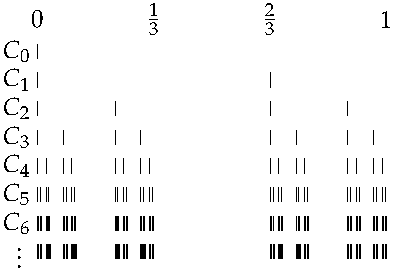
\includegraphics{cantor-similar3}
		\qquad\qquad
		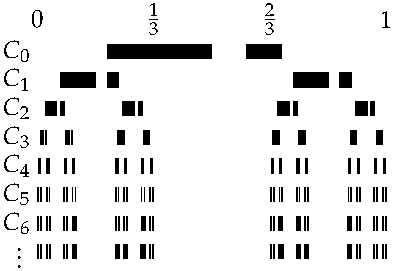
\includegraphics{cantor-similar2}
	\end{center}
\end{example*}

\goodbreak


\boldsubsubsection{Iterated Function Systems}

It certainly appears as if the Cantor set is generated by the contraction maps $S_1,S_2$ independently of the initial data $C_0$. Our main result shows in what sense this is true. The proof relies on some heavy lifting from topology so we provide only a synopsis highlighting the key points; if you've studied analysis, then several of the concepts will be familiar.

\begin{itemize}
  \item A subset of $\R^m$ is \emph{compact} if it is \emph{closed} (contains its boundary points) and \emph{bounded} (all points lie within some ball centered at the origin).
  
  \item The set of all compact subsets of $\R^m$ is a \emph{metric space} $\mathcal H$. This means that the \emph{distance} $d(X,Y)$ between two compact sets $X,Y\in\mathcal H$ may sensibly be defined, though it is a little tricky\ldots%
  \footnote{%
  	The distance function is the \emph{Hausdorff metric.} Given $Y\in\mathcal H$, and $x\in \R^n$, define $d_Y(x)=\inf_{y\in Y}\Nm{x-y}$ to be the distance from $x$ to the `nearest' point of $Y$. Define $d_X(y)$ similarly. The Hausdorff distance between $X$ and $Y$ is then
  	\[
  		d(X,Y):=\max\left\{\sup_{x\in X}d_Y(x),\sup_{y\in Y}d_X(y)\right\}
  	\]
  	Roughly speaking, find $x\in X$ which is as far away ($d_Y(x)$) as possible from $Y$ and find $y\in Y$ similarly; $d(X,Y)$ is the larger of these distances.
  }
  
  \item Since $\mathcal H$ is a metric space, we can discuss convergent sequences $(K_n)$ of compact sets
	\[
		\lim_{n\to\infty}K_n=K\iff \lim_{n\to\infty}d(K_n,K)=0
	\]
	It also makes sense to speak of Cauchy sequences in $\mathcal H$. It may be proved that $\mathcal H$ is \emph{complete}: every Cauchy sequence $(K_n)\subseteq\mathcal H$ converges to some $K\in\mathcal H$.
	
  \item The \emph{Banach Fixed Point Theorem} now applies.
	\begin{quote}
	  If $S:\mathcal H\to\mathcal H$ is a contraction mapping on a complete metric space, then $S$ has a \emph{unique fixed point}: some $F\in\mathcal H$ such that $S(F)=F$. Moreover, if $F_0\in\mathcal H$ is any initial value, then the sequence defined iteratively by $F_{k+1}:=S(F_k)$ converges to $F$.
	\end{quote}
  This powerful result has applications throughout mathematics.
\end{itemize}


\begin{thm}{}{ifs}
	Let $S_1,\ldots,S_n$ be contraction mappings on $\R^m$ with scale factors $c_1,\ldots,c_n$. Define
	\[
		S:\mathcal H\to\mathcal H\quad\text{by}\quad S(D)=\bigcup_{i=1}^nS_i(D)
	\]
	\begin{enumerate}
	  \item $S$ is a contraction mapping on $\mathcal H$ with contraction factor $c=\max(c_1,\ldots,c_n)$.
	  \item $S$ has a unique fixed set $F\in\mathcal H$ given by $F=\lim\limits_{k\to\infty} S^k(E)$ for any non-empty $E\in\mathcal H$.
	\end{enumerate}
\end{thm}

Part 1 is not difficult to prove if you're willing to work with the definition of the Hausdorff metric (try it if you're comfortable with analysis!). Part 2 is Banach's theorem.\smallbreak

The upshot is this: repeatedly applying contraction mappings to \emph{any} non-empty compact set $E$ produces a limit which is \emph{independent of $E$!} We call the limit set $F$ for \emph{fractal.} Such fractals are often called \emph{attractors}: being limit-sets, they `attract' data towards themselves.

\goodbreak


\begin{examples}{}{scarpet}
	\exstart (Cantor set Example\,\ref{ex:cantor})\lstsp The contractions $S_1(x)=\frac 13x$ and $S_2(x)=\frac 13x+\frac 23$ (on $\R$) produce a contraction mapping $S:\mathcal H\to\mathcal H$:
	\[
		\forall K\subset\R\ \text{ compact },\ S(K)=\{S_1(x),S_2(x):x\in K\}
	\]
	By Theorem \ref{thm:ifs}, $\mathcal C=\lim S^n(E)$ for \emph{any} closed bounded subset $E\subset\R$.	
	\begin{enumerate}\setcounter{enumi}{1}
	  \item[]As a nice application, one can easily find all sorts of interesting points in the Cantor set. For instance, suppose $x,y\in\R$ satisfy $y=S_1(x)$ and $x=S_2(y)$: otherwise said
		\[
			y=\frac 13 x\quad\text{and}\quad x=\frac 13(y+2)
		\]
		Since $E=\{x,y\}$ is a compact set satisfying $E\subseteq S(E)$, it follows that $E\subseteq\lim S^k(E)=\mathcal C$: both $x,y$ lie in the Cantor set! However, we easily see that $x=\frac 34$ and $y=\frac 14$, which seems paradoxical: $\frac 14$ does not lie at the end of any deleted interval (denominators of the form $3^n$) but yet the Cantor set contains no intervals. How does $\frac 14$ end up in there?!
	
		\begin{minipage}[t]{0.65\linewidth}\vspace{0pt}
			\item (Koch curve, Example\,\ref{ex:koch})\lstsp Define functions $S_i:\R^2\to\R^2$, each with scale factor $c=\frac 13$.
		\end{minipage}
		\hfill
		\begin{minipage}[t]{0.34\linewidth}\vspace{0pt}
			\flushright \href{http://www.math.uci.edu/~ndonalds/math161/koch-anim2.html}{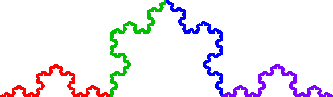
\includegraphics[scale=0.95]{koch3}}
		\end{minipage}\par
		\vspace{-27pt}
		\[
			\renewcommand\arraystretch{1.4}
			\begin{array}{l|l}
				\text{Mapping}&\text{Effect}\\\hline
				\displaystyle \textcolor{red}{S_1}(x,y)=\left(\tfrac x3,\tfrac y3\right)
				&
				\text{Scale $\frac 13$}
				\\
				\displaystyle \textcolor{Green}{S_2}(x,y)=\left(\tfrac 16x-\tfrac{\sqrt 3}6y+\tfrac 13,\tfrac{\sqrt 3}6x+\tfrac 16y\right)
				&
				\text{Scale $\frac 13$, rotate \ang{60}, translate}
				\\
				\displaystyle \textcolor{blue}{S_3}(x,y)=\left(\tfrac 16x+\tfrac{\sqrt 3}6y+\tfrac 12,\tfrac{\sqrt 3}6x-\tfrac 16y+\tfrac{\sqrt 3}6\right)
				&
				\text{Scale $\frac 13$, rotate $-\ang{60}$, translate}
				\\
				\displaystyle \textcolor{purple}{S_4}(x,y)=\left(\tfrac x3+\tfrac 23,\tfrac y3\right)
				&
				\text{Scale $\frac 13$, translate}
			\end{array}
		\]
		Applied to an initial unit line segment $E$, the image of each map is colored. The picture links to a series of animated constructions starting with different initial sets $E$.
		
		\begin{minipage}[t]{0.72\linewidth}\vspace{0pt}
			\item (Sierpiński carpet)\lstsp Eight contraction mappings produce this fractal, each reducing the whole by a (length-scale) factor of $\frac 13$.\smallbreak
			As with the Koch curve, the image links to several alternative constructions using different initial starting sets.
		\end{minipage}
		\hfill
		\begin{minipage}[t]{0.27\linewidth}\vspace{0pt}
			\flushright \href{http://www.math.uci.edu/~ndonalds/math161/sier-anim.html}{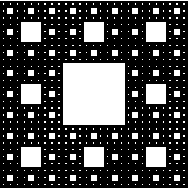
\includegraphics[scale=0.95]{sieranim2}}
		\end{minipage}\par
		
		
		\begin{minipage}[t]{0.72\linewidth}\vspace{0pt}
			\item (A Fractal Fern)\lstsp This is built from three contraction mappings:
			\begin{itemize}
				\item[$S_1$:] Scale by $\frac 34$, rotate \ang{5} clockwise, and translate by $(0,\frac 14)$
				\item[$S_2$:] Scale by $\frac 14$, rotate \ang{60} counter-clockwise, and translate by $(0,\frac 14)$
				\item[$S_3$:] Scale by $\frac 14$, rotate \ang{60} clockwise, and translate by $(0,\frac 14)$
			\end{itemize}
		\end{minipage}
		\hfill
		\begin{minipage}[t]{0.27\linewidth}\vspace{0pt}
			\flushright \href{http://www.math.uci.edu/~ndonalds/math161/fern-anim.html}{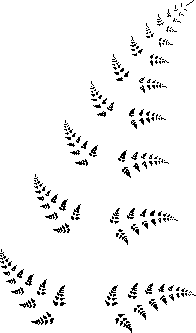
\includegraphics[scale=0.95]{fern2}}
		\end{minipage}
	\end{enumerate}
\end{examples}


\goodbreak


\begin{minipage}[t]{0.8\linewidth}\vspace{0pt}
	\boldsubsubsection{Fractal Dimension Revisited}
	
	Since Theorem \ref{thm:ifs} permits several different contraction factors, we need a new approach to fractal dimension. We ask how many disks of a given radius $\epsilon$ are required to cover a set. In the picture, the \textcolor{blue}{unit square} requires four disks of radius $\varepsilon=0.4$. For smaller $\varepsilon$, we plainly need more disks\ldots
\end{minipage}
\hfill
\begin{minipage}[t]{0.19\linewidth}\vspace{0pt}
	\flushright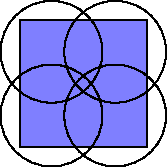
\includegraphics{epsiloncover}
\end{minipage}


\begin{defn}{}{}
	Let $K$ be a compact subset of $\R^m$.
	\begin{enumerate}
	  \item If $\varepsilon>0$, the \emph{closed $\varepsilon$-ball centered at $x\in K$} consists of the points at most a distance $\varepsilon$ from $x$:
		\[
			B_\epsilon(x)=\{y\in\R^m:d(x,y)\le\varepsilon\}
		\]
	% 	\item A finite union $\smash{\bigcup\limits_{n=1}^MB(x_n,\varepsilon)}$ is an \emph{$\varepsilon$-covering} of $A$ if $A\subseteq \smash{\bigcup\limits_{n=1}^MB(x_n,\varepsilon)}$: that is,
	% 	\[\forall x\in A,\ \exists n\ \text{ such that }\ x\in B(x_n,\varepsilon)\]
		\item The \emph{minimal $\varepsilon$-covering number} for $K$ is the smallest number of radius-$\epsilon$ balls needed to cover $K$:
		\[
			\mathcal N(K,\varepsilon)=\min\left\{M:\exists x_1,\ldots,x_M\in K\text{ with }K\subseteq \bigcup\limits_{n=1}^MB_\epsilon(x_n)\right\}
		\]
		
		\item The \emph{fractal dimension} of $K$ is the limit
		\[
			D=\lim_{\varepsilon\to 0}\frac{\log\mathcal N(K,\varepsilon)}{\log (1/\varepsilon)}
		\]
	\end{enumerate}
\end{defn}

Rigorously proving that $\cN$ and $D$ exist requires a more thorough study of topology, though a simple example should at least convince us that the definition is reasonable!

\begin{example}{}{intervalcover}
	Let $K=[0,1]$ be the interval of length 1. It is not hard to check that
	\[
		\varepsilon\ge\frac 12\iff \cN(K,\varepsilon)=1\quad\text{and}\quad 
		\frac 14\le \varepsilon<\frac 12\iff \cN(K,\varepsilon)=2
	\]
	etc. More generally, $\cN$ and $\epsilon$ are related via
	\[
		\frac 1{2\cN}\le\epsilon<\frac 1{2(\cN-1)}
	\]
	% \[\def\arraystretch{1.3}\begin{array}{c|c}
	% \text{range of }\varepsilon&\mathcal N([0,1],\epsilon)\\\hline
	% \frac 12\le \varepsilon&1\\
	% \frac 14\le\varepsilon<\frac 12&2\\
	% \frac 16\le\varepsilon<\frac 14&3\\
	% \frac 18\le\varepsilon<\frac 16&4\\
	% \frac 1{10}\le\varepsilon<\frac 18&5\\
	% \frac 1{2m}\le\varepsilon<\frac 1{2(m-1)}&m
	% \end{array}\]
	% \[\begin{array}{c|ccccccc}\def\arraystretch{1.3}
	% \text{range of }\varepsilon & [\frac 1{2m},\frac 1{2(m-1)}) & \cdots & [\frac 1{10},\frac 18) & [\frac 18,\frac 16) & [\frac 16,\frac 14) & [\frac 14,\frac 12) & [\frac 12,\infty)\\\hline
	% \mathcal N([0,1],\epsilon) & m & \cdots & 5 & 4 & 3 & 2 & 1
	% \end{array}\]
	The dimension of $K$ ($=1$) may therefore be recovered via the squeeze theorem
	\[%\frac{\log\mathcal N}{\log (2\cN)} <\frac{\log\mathcal N}{\log (1/\varepsilon)}< \frac{\log\mathcal N}{\log (2(\cN-1))}  \implies 
		D=\lim_{\epsilon\to 0}\frac{\log\mathcal N}{\log (1/\varepsilon)}=1
	\]
\end{example}



Thankfully an easier-to-visualize modification is available using boxes.

\begin{thm}{Box-counting}{}
	Let $K\subset\R^m$ be compact and cover $\R^m$ by boxes of side length $\frac 1{2^n}$. Let $\mathcal N_n(K)$ be the number of such boxes intersecting $K$. Then
	\[
		D=\lim_{n\to\infty}\frac{\log\mathcal N_n(K)}{\log 2^n}
	\]
\end{thm}


\goodbreak


We finish with a formula satisfied by the dimension of an iterated function system (Theorem \ref{thm:ifs}).

\begin{thm}{}{ifsdimension}
	Let $\{S_n\}_{n=1}^M$ be an iterated function system with attractor (limiting fractal) $F$ and where each contraction $S_n$ has scale factor $c_n\in(0,1)$. Under reasonable conditions,\footnotemark{} the fractal dimension is the unique real number $D$ satisfying
	\[
		\sum_{n=1}^Mc_n^D=1
	\]
\end{thm}

\footnotetext{%
	Roughly: the outputs of each $S_n$ meet only at boundary points; the `pieces' of the fractal cannot overlap too much.%
}


\begin{examples}{}{}
	\exstart We easily recover Definition \ref{defn:selfsim} when the scale-factors are identical $c_n=r$:
	\[
		Mr^D=1\implies D=\frac{-\log M}{\log r}=\frac{\log M}{\log (1/r)}
	\]
	\begin{enumerate}\setcounter{enumi}{1}
	  \item The fractal fern (Examples \ref{ex:scarpet}) is generated by three contraction maps with scale factors $\frac 34,\frac 14,\frac 14$. Its dimension is the solution to the equation
	  \[
	  	\left(\frac 34\right)^D+\left(\frac 14\right)^D+\left(\frac 14\right)^D=1\implies D\approx 1.3267
	  \]
	  \item Numerical approximation is usually required to find $D$, though sometimes an exact solution is possible. For instance, if $c_1=c_2=\frac 12$ and $c_3=c_4=c_5=\frac 14$, then
	  \[
	  	2\left(\frac 12\right)^D+3\left(\frac 14\right)^D=1
	  \]
	  This is quadratic in $\alpha=\left(\frac 12\right)^D$, whence
	  \[
	  	2\alpha+3\alpha^2=1\implies \alpha=\frac 13\implies D=\log_23\approx 1.584
	  \]
	\end{enumerate}
\end{examples}


\begin{minipage}[t]{0.63\linewidth}\vspace{0pt}
	\boldsubsubsection{Other methods of creating fractals}
	
	The contraction mapping approach is one of many ways to create fractals. Two other famous examples are the \href{https://en.wikipedia.org/wiki/Logistic_map}{\emph{logistic map}} (related to numerical approximations to non-linear differential equations) and the \href{https://en.wikipedia.org/wiki/Mandelbrot_set}{\emph{Mandelbrot set}} (pictured).\smallbreak
	The Mandelbrot set arises from a construction in the complex plane. For a given $c\in\C$, we iterate the function
	\[
		f_c(z)=z^2+c
	\]
	If $f(f(f(\cdots f(c)\cdots)))$ remains bounded, no matter how many times $f$ is applied, then $c$ lies in the Mandelbrot set.\smallbreak
	Much better pictures and trippy videos can be found online\ldots
\end{minipage}
\hfill
\begin{minipage}[t]{0.35\linewidth}\vspace{0pt}
	\flushright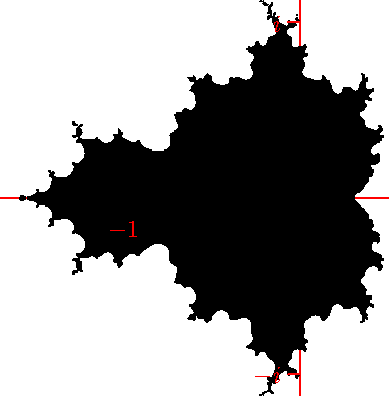
\includegraphics[scale=0.9]{mandelbrot}
\end{minipage}
\goodbreak



\begin{exercises}
	\exstart Let $S_1(x)=\frac 13 x$ and $S_2(x)=\frac 13x+\frac 23$ be the contraction mappings defining the Cantor set and suppose $x,y,z\in\R$ satisfy
	\[
		y=S_1(x),\qquad z=S_2(y),\qquad x=S_2(z)
	\]
	Show that $x,y,z$ lie in the Cantor set, and find their values.
	
	  
	\begin{enumerate}\setcounter{enumi}{1}
	  \item We illustrate Banach's theorem.
	  \begin{enumerate}
	    \item The contraction mapping $S(x)=\frac 13x+\frac 23$ (on $\R$) plainly has unique fixed point $x=1$ ($S(x)=x\Longleftrightarrow x=1$). If $x_0\in\R$ is given and $x_{n+1}:=S(x_n)$ for all $n\in\N_0$, prove that $x_n=1+(x_0-1)3^{-n}$ and thus conclude that $\lim x_n=1$.
	    \item Repeat part (a) for any linear polynomial $S(x)=cx+d$ where $\nm c<1$. 
	  \end{enumerate}
	  
	  
	  \item The construction of a Cantor-type set starts by removing the open intervals $(0.1,0.2)$ and $(0.6,0.8)$ from the unit interval.
	  \begin{enumerate}
	    \item Sketch the first three iterations of this fractal.
	    \item This construction may be described using three contraction mappings; what are they?
	    \item State an equation satisfied by the dimension $D$ of the set and use a computer algebra package to estimate its value.
	  \end{enumerate}
	  
		\item A variation on the Koch curve is constructed using the following contraction mappings. Each is built by first scaling the whole picture by a factor $c$, rotating the picture through an angle counter-clockwise, and then translating the picture by adding a constant. The resulting fractal is drawn.\par  
	  \begin{minipage}{0.52\linewidth}
		  \qquad$\displaystyle\def\arraystretch{1.2}
		  \begin{array}{c|c|c|c}
			  \text{map}&\text{scale}&\text{rotate}&\text{translate (add $(x,y)$)}\\\hline
			  S_1&\frac 12&0&0\\
			  S_2&\frac 14&\ang{90}&(\frac 12,0)\\
			  S_3&\frac 14&0&(\frac 12,\frac 14)\\
			  S_4&\frac 14&-\ang{90}&(\frac 34,\frac 14)\\
			  S_5&\frac 14&0&(\frac 34,0)
		  \end{array}$
	  \end{minipage}
	  \hfill
	  \begin{minipage}{0.47\linewidth}
	  	\flushright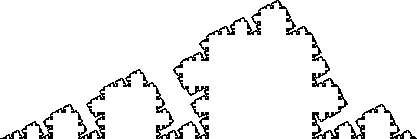
\includegraphics{fractal}
	  \end{minipage}\par
	  \begin{enumerate}
	    \item Suppose you start with the straight line segment from $(0,0)$ to $(1,0)$. Draw the first two iterations of the fractal's construction.
	    \item The dimension of the fractal is the unique solution $D$ to the equation
	    \[
	    	\left(\frac 12\right)^D+\left(\frac 14\right)^D+\left(\frac 14\right)^D+\left(\frac 14\right)^D+\left(\frac 14\right)^D=1
	    \]
	    By observing that $\frac 14=\left(\frac 12\right)^2$, convert this to a quadratic equation in the variable $\alpha:=\left(\frac 12\right)^D$. Hence compute the dimension of the fractal.
	    \item The dimension computed in part (b) is \emph{larger} than the dimension $\frac{\log 4}{\log 3}$ of the Koch curve. Explain what this means.
	  \end{enumerate}
	
	
		\item Verify the details of Example \ref{ex:intervalcover}, including the computation of the limit.
	
		\item Given constants $0\le c_1,\ldots,c_n<1$, use the intermediate value theorem from calculus to prove that the value $D$ in Theorem \ref{thm:ifsdimension} exists and is unique.
		
	\end{enumerate}
\end{exercises}